\documentclass[english]{book}
\newcommand{\G}{\overline{C_{2k-1}}}
\usepackage[latin9]{inputenc}
\usepackage{amsmath}
\usepackage{amssymb}
\usepackage{lmodern}
\usepackage{mathtools}
\usepackage[inline]{enumitem}
\usepackage{multicol}
%\usepackage{natbib}
%\bibliographystyle{plainnat}
%\setcitestyle{authoryear,open={(},close={)}}content...
\let\avec=\vec
\renewcommand\vec{\mathbf}
\renewcommand{\d}[1]{\ensuremath{\operatorname{d}\!{#1}}}
\newcommand{\pydx}[2]{\frac{\partial #1}{\partial #2}}
\newcommand{\dydx}[2]{\frac{\d #1}{\d #2}}
\newcommand{\ddx}[1]{\frac{\d{}}{\d{#1}}}
\newcommand{\hk}{\hat{K}}
\newcommand{\hl}{\hat{\lambda}}
\newcommand{\ol}{\overline{\lambda}}
\newcommand{\om}{\overline{\mu}}
\newcommand{\all}{\text{all }}
\newcommand{\valph}{\vec{\alpha}}
\newcommand{\vbet}{\vec{\beta}}
\newcommand{\vT}{\vec{T}}
\newcommand{\vN}{\vec{N}}
\newcommand{\vB}{\vec{B}}
\newcommand{\vX}{\vec{X}}
\newcommand{\vx}{\vec {x}}
\newcommand{\vn}{\vec{n}}
\newcommand{\vxs}{\vec {x}^*}
\newcommand{\vV}{\vec{V}}
\newcommand{\vTa}{\vec{T}_\alpha}
\newcommand{\vNa}{\vec{N}_\alpha}
\newcommand{\vBa}{\vec{B}_\alpha}
\newcommand{\vTb}{\vec{T}_\beta}
\newcommand{\vNb}{\vec{N}_\beta}
\newcommand{\vBb}{\vec{B}_\beta}
\newcommand{\bvT}{\bar{\vT}}
\newcommand{\ka}{\kappa_\alpha}
\newcommand{\ta}{\tau_\alpha}
\newcommand{\kb}{\kappa_\beta}
\newcommand{\tb}{\tau_\beta}
\newcommand{\hth}{\hat{\theta}}
\newcommand{\evat}[3]{\left. #1\right|_{#2}^{#3}}
\newcommand{\prompt}[1]{\begin{prompt*}
		#1
\end{prompt*}}
\newcommand{\vy}{\vec{y}}
\DeclareMathOperator{\sech}{sech}
\DeclarePairedDelimiter\abs{\lvert}{\rvert}%
\DeclarePairedDelimiter\norm{\lVert}{\rVert}%
%\newcommand{\dis}[1]{\begin{align*}
%	#1
%	\end{align*}}
\newcommand{\dis}[1]{$\displaystyle{#1}$}
\newcommand{\LL}{\mathcal{L}}
\newcommand{\RR}{\mathbb{R}}
\newcommand{\CC}{\mathbb{C}}
\newcommand{\NN}{\mathbb{N}}
\newcommand{\ZZ}{\mathbb{Z}}
\newcommand{\QQ}{\mathbb{Q}}
\newcommand{\Ss}{\mathcal{S}}
\newcommand{\BB}{\mathcal{B}}
\usepackage{graphicx}
\setlength{\columnseprule}{1pt}

% Swap the definition of \abs* and \norm*, so that \abs
% and \norm resizes the size \dis{\tan (\pi/6)}of the brackets, and the ake no more than 5 minutes on question 0}
%%\prob{0}\textbf{Oops! Looks like the American dollar went belly-up last week, and as a result, society has completely collapsed across the globe!\footnote{Maybe next time, consider using something less volatile as the world's reserve currency\textemdash for now though, tough luck.} Eventually, maybe civilization will rebuild, but for now, it's total chaos\textemdash there's no longer such thing as currency, half the city is on fire, and the police and army have both fractured into a complicated web of warring factions. You and your group have to band up to survive. In the space below, determine a) what your top priorities for survival should be in the immediate term and b) what role each member will play for your team.}
% starred version does not.
%\makeatletter
%\let\oldabs\abs
%\def\abs{\@ifstar{\oldabs}{\oldabs*}}
%content...
%\let\oldnorm\norm
%\def\norm{\@ifstar{\oldnorm}{\oldnorm*}}
%\makeatother
\newenvironment{subproof}[1][\proofname]{%
	\renewcommand{\qedsymbol}{$\blacksquare$}%
	\begin{proof}[#1]%
	}{%
	\end{proof}%
}

\usepackage{centernot}
\usepackage{dirtytalk}
\usepackage{calc}
%\newcommand{\prob}[1]{\setcounter{section}{#1-1}\section{}}
%\newcommand{\prt}[1]{\setcounter{subsection}{#1-1}\subsection{}}
%\newcommand{\pprt}[1]{{\textit{{#1}.)}}\newline}

\usepackage[]{titlesec}
\usepackage{etoolbox}
%\titlelabel{\thetitle.)\quad}
\DeclarePairedDelimiter\floor{\lfloor}{\rfloor}
\makeatletter

%\newcommand*\pFqskip{8mu}
%\catcode`,\activecontent...
%\newcommand*\pFq{\begingroup
%	\catcode`\,\active
%	\def ,{\mskip\pFqskip\relax}%
%	\dopFq
%}
%\catcode`\,12
%\def\dopFq#1#2#3#4#5{%
%	{}_{#1}F_{#2}\biggl(\genf\dis{\tan (\pi/6)}rac..{0pt}{}{#3}{#4}|#5\biggr
%	)%
%	\endgroup
%}
\def\res{\mathop{Res}\limits}
% Symbols \wedge and \vee from mathabx
% \DeclareFontFamily{U}{matha}{\hyphenchar\font45}
% \DeclareFontShape{U}{matha}{m}{n}{content...
%       <5> <6> <7> <8> <9> <\dis{\tan (\pi/6)}10> gen * matha
%       <10.95> matha10 <12> <14.4> <17.28> <20.74> <24.88> matha12
%       }{}
% \DeclareSymbolFont{matha}{U}{matha}{m}{n}ake no more than 5 minutes on question 0}
%%\prob{0}\textbf{Oops! Looks like the American dollar went belly-up last week, and as a result, society has completely collapsed across the globe!\footnote{Maybe next time, consider using something less volatile as the world's reserve currency\textemdash for now though, tough luck.} Eventually, maybe civilization will rebuild, but for now, it's total chaos\textemdash there's no longer such thing as currency, half the city is on fire, and the police and army have both fractured into a complicated web of warring factions. You and your group have to band up to survive. In the space below, determine a) what your top priorities for survival should be in the immediate term and b) what role each member will play for your team.}
% \DeclareMathSymbol{\wedge}         {2}{matha}{"5E}
% \DeclareMathSymbol{\vee}           {2}{matha}{"5F}content...
% \makeatother

%\titlelabel{(\thesubsection)}
%\titlelabel{(\thesubsection)\quad}
\usepackage{listings}
%\lstloadlanguages{[5.2]Mathematica}
\usepackage{babel}
\newcommand{\ffac}[2]{{(#1)}^{\underline{#2}}}
\usepackage{color}
\usepackage{amsthm}
\newtheorem{theorem}{Theorem}[section]
%\newtheorem*{theorem*}{Theorem}[section]
\newtheorem{conj}[theorem]{Conjecture}
\newtheorem{corollary}[theorem]{Corollary}
\newtheorem{example}[theorem]{Example}
\newtheorem{lemma}[theorem]{Lemma}
\newtheorem*{lemma*}{Lemma}


\newtheorem{proposition}[theorem]{Proposition}
\newtheorem*{prop*}{Proposition}
\newtheorem*{corollary*}{Corollary}


\newtheorem*{claim*}{Claim}
\newcommand{\claim}[1]{\begin{claim*} #1\end{claim*}}
%organizing theorem environments by style--by the way, should we really have definitions (and notations I guess) in proposition style? it makes SO much of our text italicized, which is weird.
\theoremstyle{remark}
\newtheorem{remark}{Remark}[theorem]
\newtheorem{caution}{Caution}[theorem]

\theoremstyle{definition}
\newtheorem{excs}{Exercise}[chapter]
\newtheorem{hint}{Hint}[excs]
%\newtheorem{prbm}[excs]{Problem}
\newtheorem{exle}[theorem]{Example}
\newtheorem{definition}[theorem]{Definition}
\newtheorem{notation}[theorem]{Notation}
\newtheorem*{notation*}{Notation}
\newtheorem*{goal}{Goal}
\newtheorem*{next week}{Next Week}
\newtheorem{fact}[theorem]{Fact}
\newtheorem{fifact}[theorem]{Foundationally Important Fact}
\renewcommand{\theexcs}{\arabic{chapter}.\Alph{excs}}
%FINAL
\newcommand{\due}{Summer 2018} 
\RequirePackage{geometry}
\geometry{margin=.7in}
\usepackage{todonotes}
\title{Calc 1.5 Notes}
\author{David DeMark}
\date{\due}
\usepackage{fancyhdr}
\usepackage{nameref}
\pagestyle{fancy}
\fancyhf{}
\lhead{Calc 1.5 Notes}
\rhead{\due}
\chead{\nouppercase\leftmark}
\cfoot{\thepage}
% %%
%%
%%
%DRAFT

%\usepackage[left=1cm,right=4.5cm,top=2cm,bottom=1.5cm,marginparwidth=4cm]{geometry}
%\usepackage{todonotes}inparaenum
% \title{MATH 8669 Homework 4-DRAFT}
% \usepackage{fancyhdr}
% \pagestyle{fancy}
% \fancyhf{}\dis{\tan (\pi/6)}
% \rhead{David DeMark}
% \lhead{MATH 8669-Homework 4-DRAFT}
% \cfoot{\thepage}

%PROBLEM SPEFICIC

\newcommand{\lint}{\underline{\int}}
\newcommand{\uint}{\overline{\int}}
\newcommand{\hfi}{\hat{f}^{-1}}
\newcommand{\tfi}{\tilde{f}^{-1}}
\newcommand{\tsi}{\tilde{f}^{-1}}
\newcommand{\PP}{\mathcal{P}}
\newcommand{\nin}{\centernot\in}
\newcommand{\seq}[1]{({#1}_n)_{n\geq 1}}
\usepackage{array}
\newcolumntype{M}[1]{>{\centering\arraybackslash}m{#1}}
\newcolumntype{N}{@{}m{0pt}@{}}
\input ArtNouvc.fd
\newcommand*\initfamily{\usefont{U}{ArtNouvc}{xl}{n}}
\newcommand{\ansl}{~\underline{\hspace{1.5cm}}}
\usepackage{pgfplots}
\pgfplotsset{my style/.append style={axis x line=middle, axis y line=
		middle, xlabel={$x$}, ylabel={$y$}, axis equal,width=\textwidth }}
\pgfplotsset{every x tick label/.append style={font=\small, yshift=0.5ex}}
\pgfplotsset{every y tick label/.append style={font=\small, xshift=0.5ex}}
%\usepackage{paralist}
\newcommand{\dlim}{\displaystyle\lim}
\begin{document}
\maketitle
\chapter{Euler's Formula \& Limits I}
\setcounter{section}{-1}
\section{Euler's Formula}
\begin{goal} Use Euler's Formula (Theorem \ref{thm:eufl}) to derive any number of trig identities.
	\end{goal}
\emph{Note that this isn't actually part of the standard pre-calc curriculum, but it is an immensely powerful tool which simplifies down quite a bit of pre-calc\textemdash frankly, it's almost offensive that this isn't taught during pre-calc. We may be able to prove Theorem \ref{thm:eufl} using Taylor series some time in August, but for now we'll need to just trust Euler on it.}

We'll be using the following fact over and over throughout this section:
\begin{fact}
	For any (real, complex, or otherwise!) $a,b,c$, we have that $a^b*a^c=a^{b+c}$.
\end{fact}

\begin{definition}
	Recall the imaginary number $i:=\sqrt{-1}$. 
\end{definition}

\begin{theorem}
\label{thm:eufl} For any real number $\theta$, $$e^{i\theta}=\cos(\theta)+i\sin(\theta)$$
\end{theorem}
\begin{caution}
	This is only true in radians! And is a compelling reason never to use degrees for much of anything\textellipsis
\end{caution}
\begin{fact}\label{fact:cplx=}
	We let $w=a+ib$ and $z=c+id$ be complex numbers (that is $w,z\in \CC$) with $a,b,c,d$ all real numbers (that is, $a,b,c,d\in \RR$). Then, $w=z$ if and only if $a=c$ and $b=d$.
\end{fact}

This is a somewhat obvious fact, but it will prove extremely useful\textemdash basically, if we can find two different ways to write the same complex number, we can then conclude that the real parts and the imaginary parts must be the same (because it's the same number!). We'll use this fact to show quite a few trig identities.

\begin{exle} Let $\theta$ be any real number.\label{ex1.0}
	Find formulas for $\sin(2\theta)$ and $\cos(2\theta)$ in terms of $\sin(\theta)$ and $\cos(\theta)$.
\end{exle}
\begin{proof}[Response]
We use Euler's Formula (Theorem \ref{thm:eufl}) to write $$e^{i(2\theta)}=\cos(2\theta)+i\sin (2\theta).$$
However, we also have by properties of exponentiation that $e^{i(2\theta)}=e^{2(i\theta)}=(e^{i\theta})^2$, and note that we already know how to expand out $e^{i\theta}$ (once again by Theorem \ref{thm:eufl}). That is, we can write
\begin{align*}e^{i(2\theta)}&=(e^{i\theta})^2\\
&=(\cos (\theta)+i\sin (\theta))^2\\
&=\cos^2(\theta) +2i\cos(\theta)\sin(\theta)+(i\sin (\theta))^2\\
&=(\cos^2\theta -\sin ^2\theta)+i(2\cos(\theta)\sin(\theta))
\end{align*}
Now, we've written the same complex number two different ways:
\begin{align*}e^{i(2\theta)}&=\cos(2\theta)+i\sin (2\theta)\\&=(\cos^2(\theta) -\sin ^2(\theta))+i(2\cos(\theta)\sin(\theta))\end{align*}
Thus, we can use Fact \ref{fact:cplx=} to now write that $\cos(2\theta)=cos^2(\theta)-\sin^2(\theta)$, and $\sin(2\theta)=2\cos (\theta)\sin(\theta).$
\end{proof}
\begin{excs}
Simplify the expression $e^{i\pi}+1$
\end{excs}
\begin{excs}
	Use the same techniques as in Example \ref{ex1.0} to find formulas for $\cos(3\theta)$ and $\sin(3\theta)$ in terms of $\cos(\theta)$ and $\sin(\theta)$. 
\end{excs}
\begin{excs} Let $\theta_1$ and $\theta_2$ be real numbers.
	Use the same techniques as in Example \ref{ex1.0} to find formulas for $\cos(\theta_1+\theta_2)$ and $\sin(\theta_1+\theta_2)$ in terms of $\sin(\theta_1)$, $\sin(\theta_2)$, $\cos(\theta_1)$, and $\cos(\theta_2)$. 
\end{excs}
\begin{excs}
	We know that in general, for any $x$, \begin{equation}e^x*e^{-x}=1.\label{eqrec}\end{equation}
	This is still true if $x$ is imaginary (or complex for that matter). Let $x=i\theta$. Reinterpret equation \eqref{eqrec} in terms of $\sin(\theta)$ and $\cos(\theta)$. What familiar trigonometric identity do we recover? (Hint: what symmetries do $\cos$ and $\sin$ have?)
\end{excs}
\section{Limits I: Formal Definition \& First Properties}
See: Stewart, \S2.4.
\begin{goal}
	Understand limits in terms of formal properties, prove basic facts regarding them.
\end{goal}
\begin{next week}
Use these properties to do a bunch of more concrete limit computations, possibly start out derivatives.
\end{next week}
\begin{definition}\label{def:lim}
	Let $f$ be a function on the real numbers, and let $a$ and $L$ be real numbers. We say $\displaystyle\lim_{x\to a}f(x)=L$ if for any real number $\epsilon>0$, there exists some real number $\delta>0$ such that if $0<\abs{x-a}<\delta$, then $\abs{f(x)-L}<\epsilon$.
\end{definition}
\begin{remark}
	$\epsilon$ is the Greek letter \emph{epsilon.} $\delta$ is the Greek letter \emph{delta.}
\end{remark}
\begin{remark}
Let's unpack that definition a bit. First, keep in mind that we should think of $\abs{x-a}$ as the \emph{distance} between $x$ and $a$. When we say \say{for any $\epsilon$, there exists a $\delta$,} that means that if \emph{we are given} some number $\epsilon$, then (theoretically) we can find some number $\delta$ with the property that if $x$ is \say{less than $\delta$ away from $a$,} then $f(x)$ is \say{less than $\epsilon$ away from $L$.} 

To illustrate this more concretely, let's add in some literal illustrations. Suppose we have the curve $y=f(x)$ as in figure \ref{fig:1graph1}, and suppose we are considering the statement $\displaystyle\lim_{x\to a} f(x)=L$.
\begin{figure}[h!]\centering
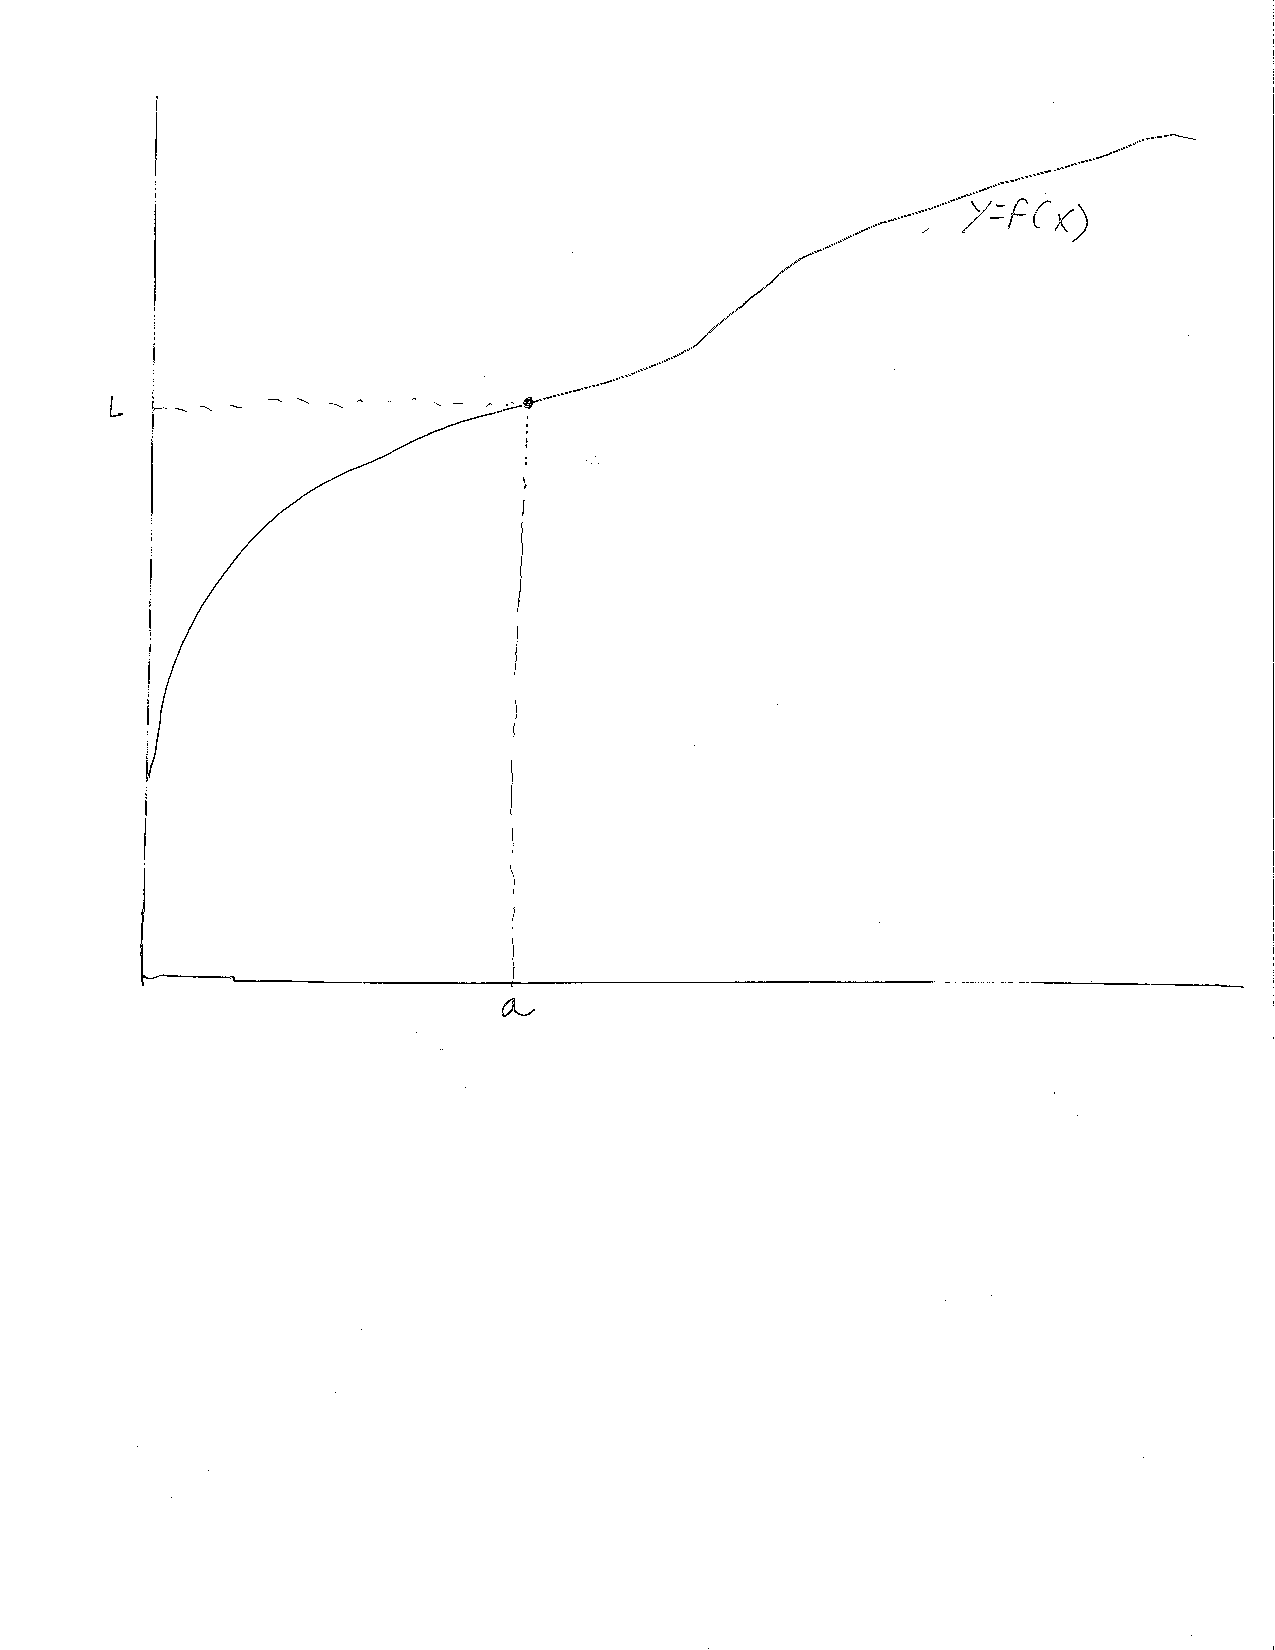
\includegraphics[scale=0.5,trim={0 4in 10mm 0},clip]{1graph1} \caption{The graph of $y=f(x)$ with $x=a$ and $y=L$ drawn in.\label{fig:1graph1}}
\end{figure}

Now, suppose we are given some real number $\epsilon>0$. $\epsilon$ corresponds to some region around $L$ on the $y$-axis (the region where $\abs{y-L}<\epsilon$). That region is drawn in red in figure \ref{fig:1graph2}

\begin{figure}[h!]\centering
	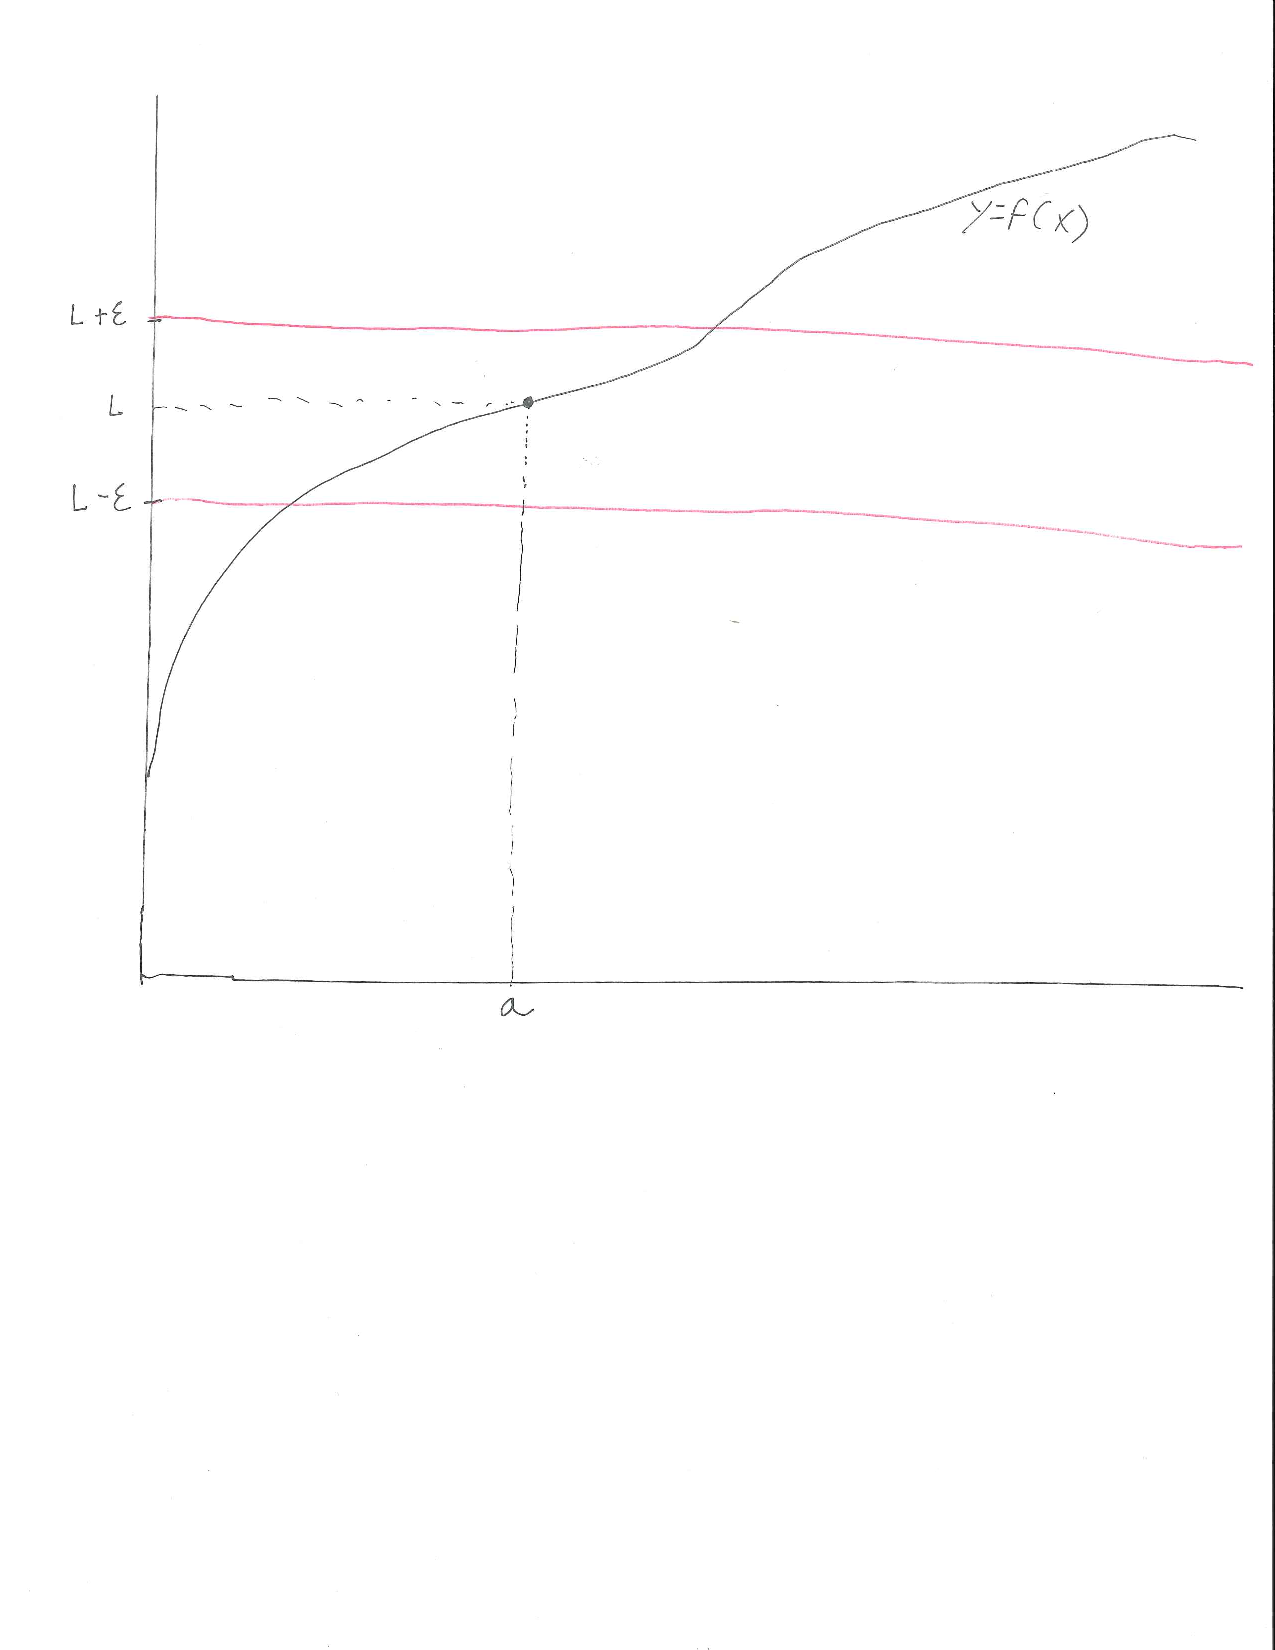
\includegraphics[scale=0.5,trim={0 4in 10mm 0},clip]{1graph2} \caption{The graph of $y=f(x)$ with the vertical region between $L-\epsilon$ and $L+\epsilon$ drawn in.\label{fig:1graph2}}
\end{figure}

\newpage Given such an $\epsilon$, we need to find some horizontal region around $x=a$ such that for any $x$ in that region, $f(x)$ is \say{close enough} to $L$. We can see from the graph that such a region indeed exists\textemdash note the part of the curve which sits between the two red lines. We choose some $\delta$ such that everything between $a-\delta$ and $a+\delta$ (that is, all $x$ with $\abs{x-a}<\delta$) has its corresponding point on the curve between $L-\epsilon$ and $L+\epsilon$. Such a $\delta$ and the corresponding region around $x=a$ is drawn in figure \ref{fig:1graph3}.

\begin{figure}[h!]\centering
	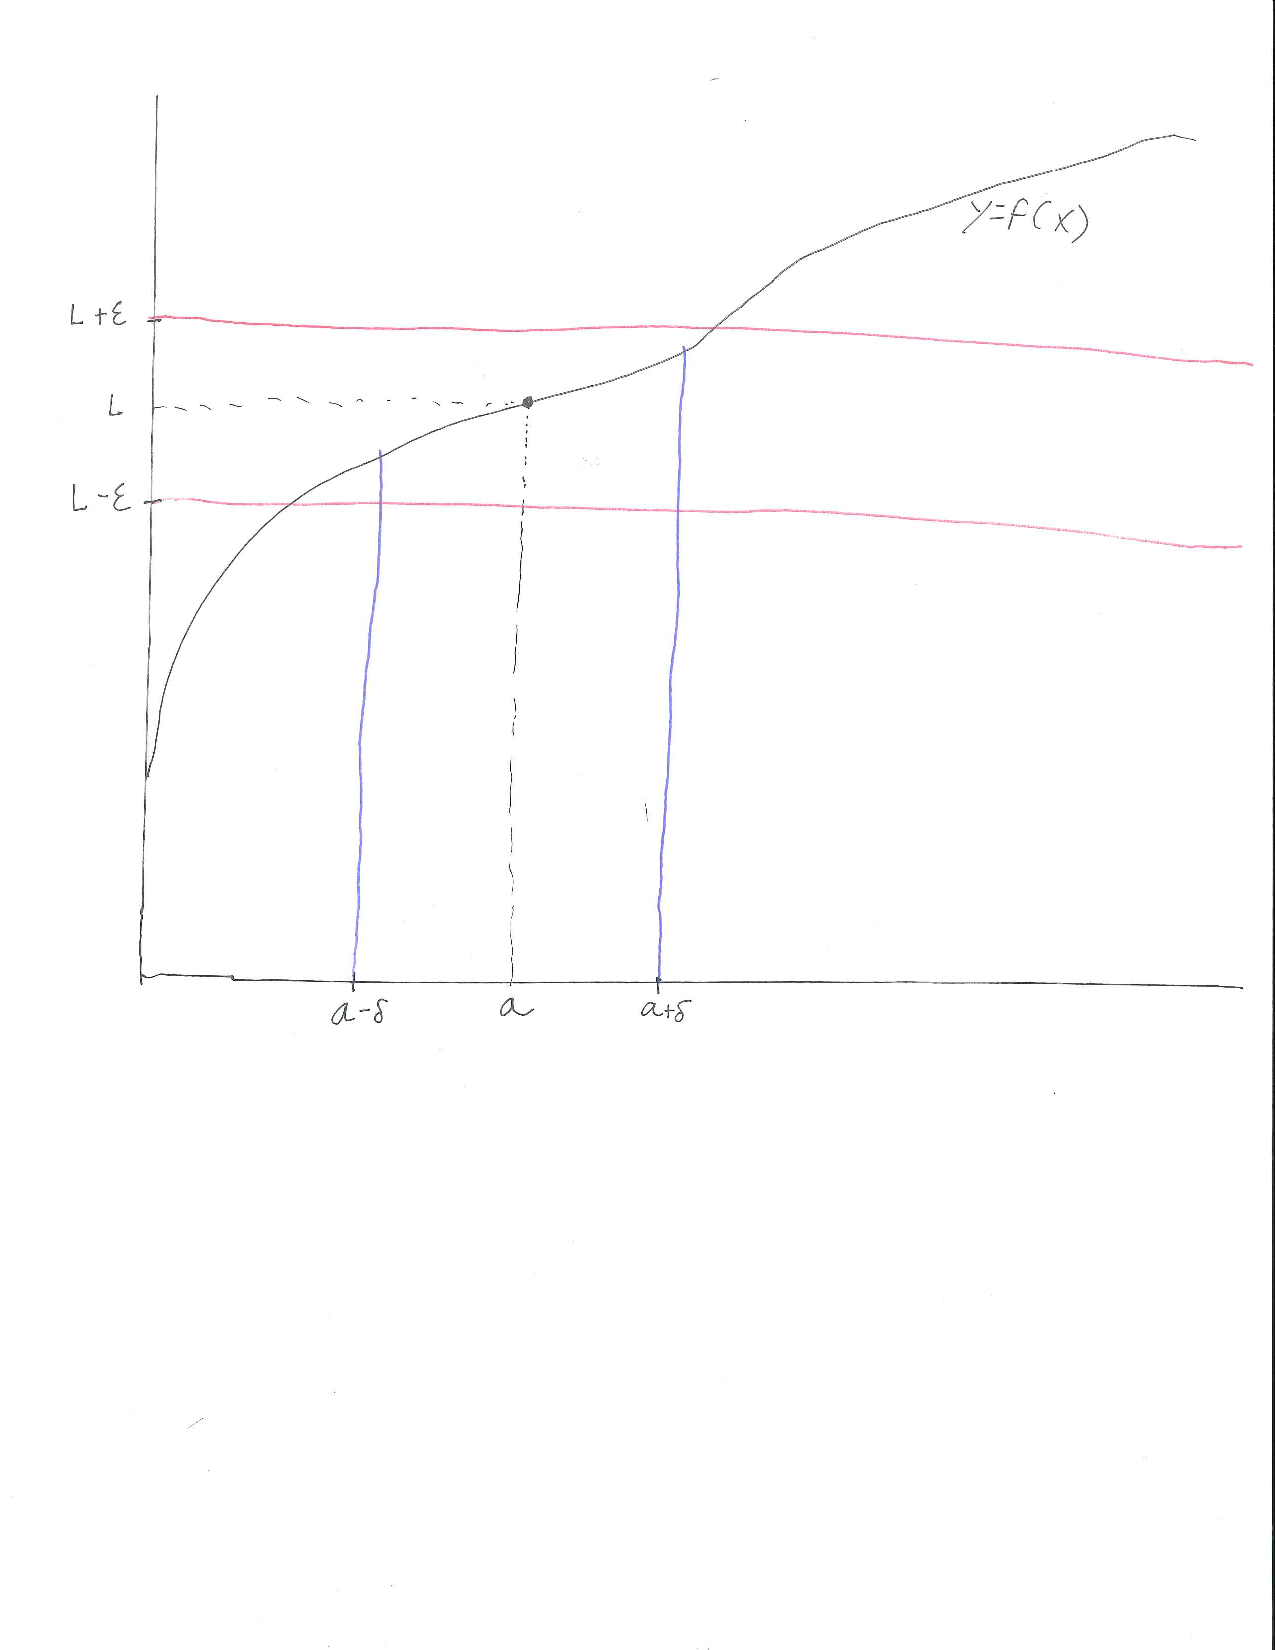
\includegraphics[scale=0.5,trim={0 4in 10mm 0},clip]{1graph3} \caption{The graph of $y=f(x)$, now with a horizontal region around $x=a$.\label{fig:1graph3}}
\end{figure}

Note that we could have chosen a different $\delta$\textemdash in particular, any smaller $\delta$ would work. Also note that we would not be done after just finding this one $\delta$\textemdash we must find such a $\delta$ for \emph{any} $\epsilon$, no matter how small\textemdash in other words, we must repeat this process infinitely many times! As that would take all day (as well as all of the other days), in practice we almost always do this abstractly (for some \emph{general} $\epsilon$) instead of case-by-case, as in Example \ref{ex:1lin}.
\end{remark}
\begin{exle}\label{ex:1lin}
	Use Definition \ref{def:lim} to show that $\displaystyle\lim_{x\to 2} 4x-3=5$.
\end{exle}
\begin{proof}[Response]
	 Let $x$ be arbitrary (that is, let it be any real number). Let's try writing out $f(x)-f(2)$.
	 \begin{align*}
	 	f(x)-f(2)&=(4x-3)-(4(2)-3)\\
	 	&=4x-3-4(2)+3\\
	 	&=4(x-2)
	 \end{align*}
%	 Thus, if we let $d=\abs{x-2}$, we have that $\abs{f(x)-f(2)}=\abs{4(x-2)}=4d$.
 Now, suppose we are given some $\epsilon>0$. We need to choose a $\delta$ such that if $\abs{x-2}<\delta$, then $\abs{f(x)-f(2)}<\epsilon$. But as we just saw, as long as we pick $0<\delta<\epsilon/4$, we get that if $\abs{x-2}<\delta$, then $\abs{f(x)-f(2)}=\abs{4(x-2)}=4\abs{x-2}<4\delta<4(\epsilon/4)=\epsilon$. So indeed, $\dlim_{x\to 2}(4x-3)=5$. 
\end{proof}

\begin{excs}
	Use the techniques of Example \ref{ex:1lin} to show that $$\lim_{x\to 3}5x-6=9$$
\end{excs}
\begin{excs}
	Or if that's too boring, use the techniques of Example \ref{ex:1lin} to show that $$\lim_{x\to a}mx+b=ma+b$$. 
\end{excs}
\subsection{Limits at/to infinity}
\begin{definition}\label{def:limto}
	We say that $\dlim_{x\to a}f(x)=\infty$ if for any real number $N$, there exists a real number $\delta>0$ such that if $0<\abs{x-a}<\delta$, then $f(x)>N$. 
\end{definition}
\begin{remark}
	Basically, the way this differs from \ref{def:lim} is defining \say{closeness to infinity.} That is, we say that $f$ \say{approaches infinity} when for any number $N$ (no matter how large!) there is a region surrounding $x=a$ where $f(x)>N$ (replacing the condition $\abs{f(x)-L}<\epsilon$).
\end{remark}
\begin{definition}\label{def:limat}
We say that $\dlim_{x\to \infty} f(x)=L$ if for any $\epsilon>0$, there exists some real number $R$ such that for all $x>R$, $\abs{f(x)-L}<\epsilon$
\end{definition}
\begin{remark}
	Once again, let's unpack this a bit. Suppose we are considering the graph of $y=f(x)$ as in figure \ref{fig:1graph4} and wish to show that $\dlim_{x\to \infty} f(x)=L$. 
	\begin{figure}[h!]\centering
		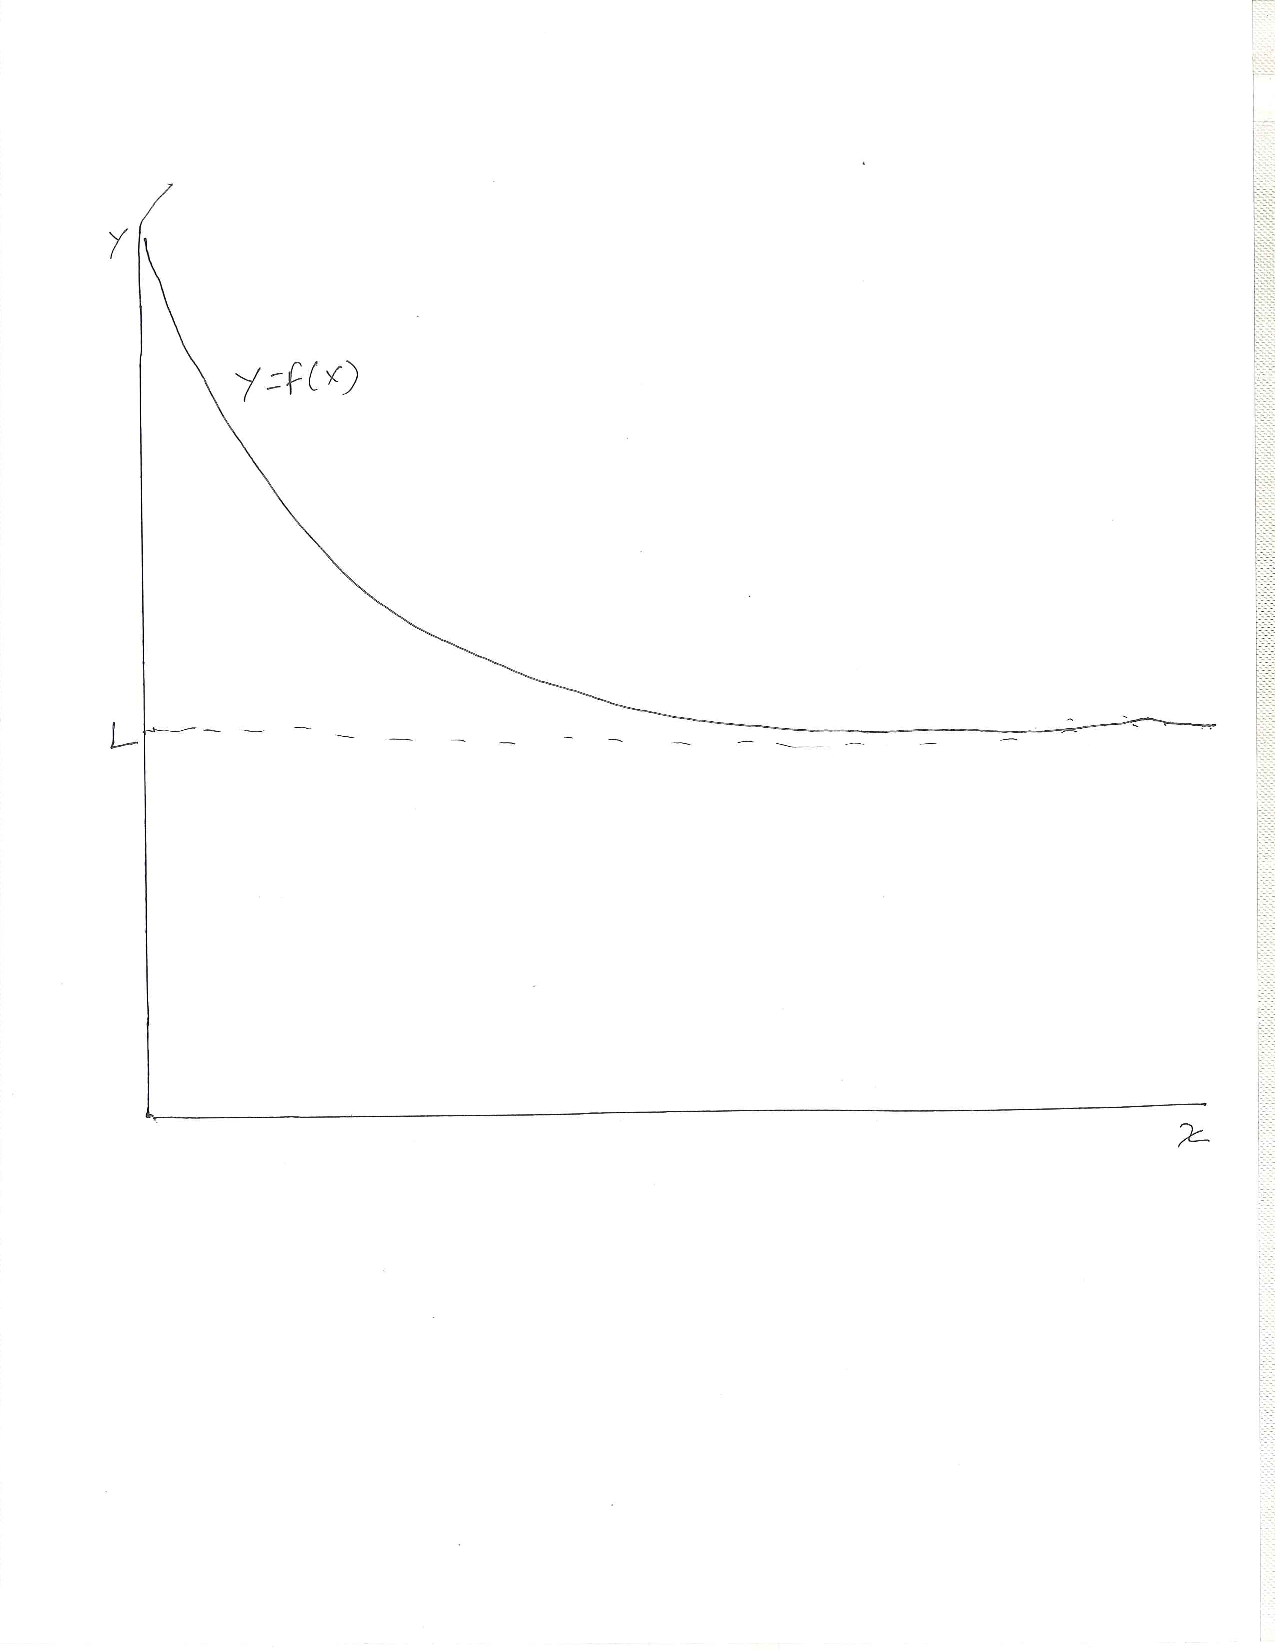
\includegraphics[scale=0.45,trim={0 3.3in 12mm 36mm},clip]{1graph4} \caption{The graph of $y=f(x)$ with $y=L$ drawn in.\label{fig:1graph4}}
	\end{figure}

Now suppose we are once again given some $\epsilon>0$. In Figure \ref{fig:1graph5}, we draw in the region on the $y$-axis of all points $y$ with $\abs{y-L}<\epsilon$ in red.
\begin{figure}[h!]\centering
	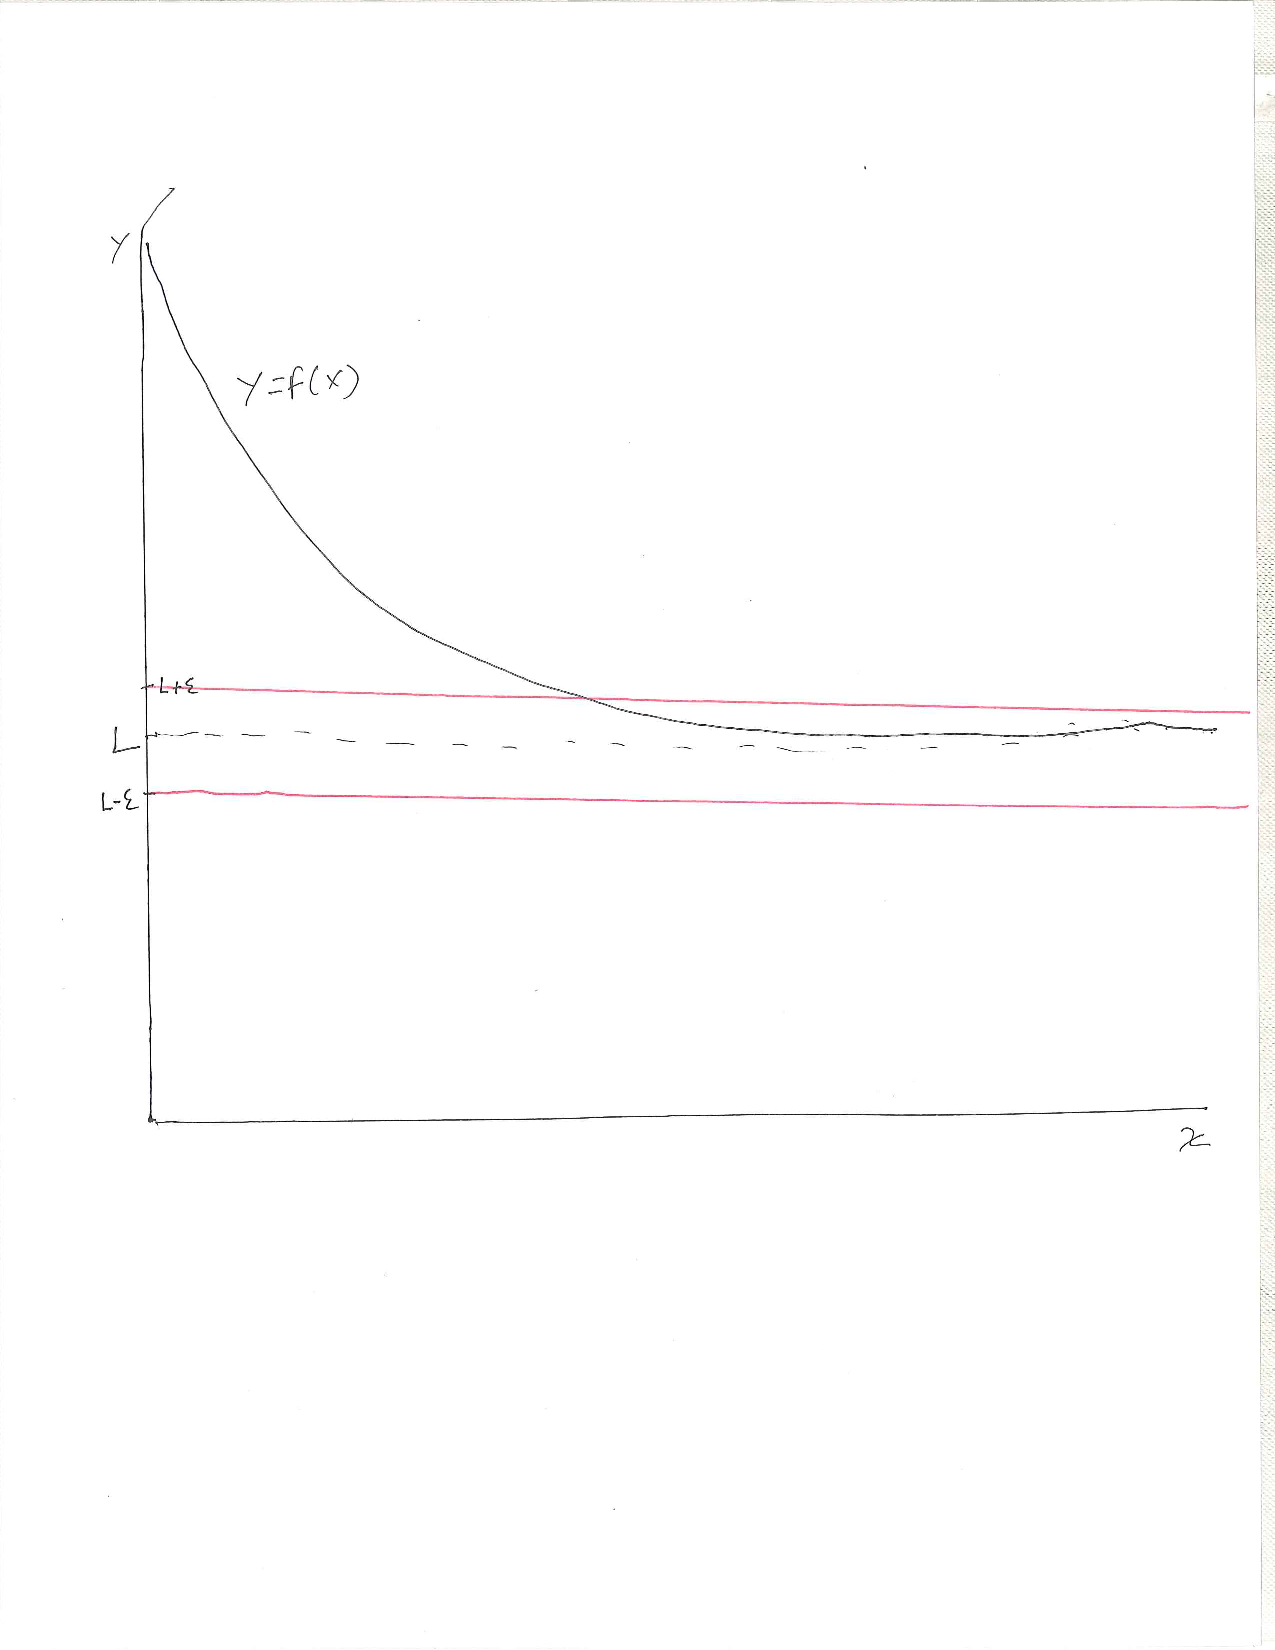
\includegraphics[scale=0.5,trim={0 3.3in 12mm 36mm},clip]{1graph5} \caption{The graph of $y=f(x)$ with $y=L$ and the surrounding region of radius $\epsilon$ drawn in.\label{fig:1graph5}}
\end{figure}
\newpage
We need to find some $R$ such that for all $x$ to the right of $R$, the graph of the function stays within the two red lines. However, we may indeed find such an $R$ (assuming the function isn't too badly behaved to the right of our frame). This $R$ is inserted in figure \ref{fig:1graph6}.

\begin{figure}[h!]\centering
	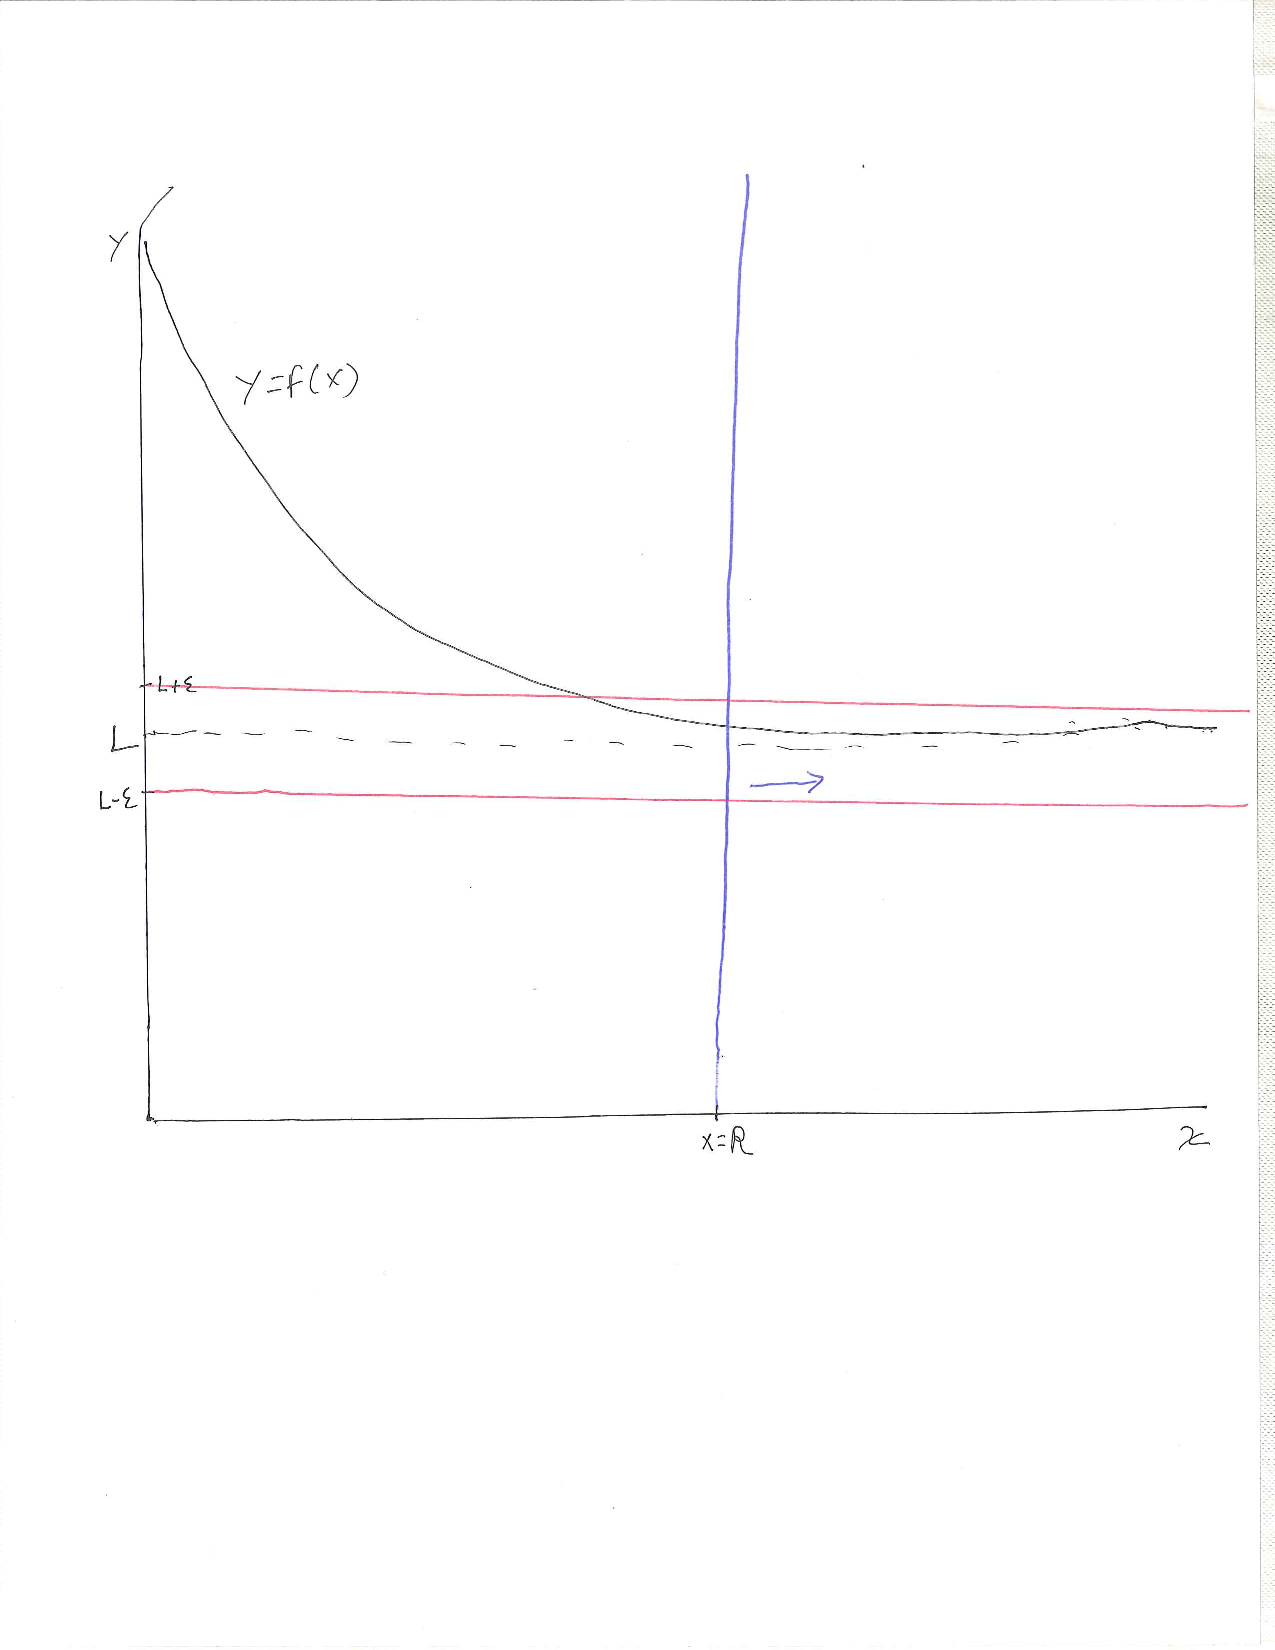
\includegraphics[scale=0.5,trim={0 3.3in 12mm 36mm},clip]{1graph6} \caption{The graph of $y=f(x)$ with $y=L$ drawn in.\label{fig:1graph6}}
\end{figure}

Of course, once more, we wouldn't actually be done once we had found this $x$-coordinate $R$\textemdash we must do so for \emph{any} possible $\epsilon$, no matter how small.
\end{remark}
\begin{excs}
	Rewrite Definitions \ref{def:limto} and \ref{def:limat} replacing $\infty$ with $-\infty$ and making the appropriate other adjustments.
\end{excs}
\begin{excs}
Combine definitions \ref{def:limat} and \ref{def:limto} in order to define what it means to say that $\dlim_{x\to \infty}f(x)=\infty$. (Hint: read ahead to the next example if you're having trouble). You don't have to write it out, but also convince yourself that you'd be able to do the same for $\dlim_{x\to -\infty}f(x)=\infty$, $\dlim_{x\to \infty} f(x)=-\infty$ and $\dlim_{x\to -\infty} f(x)=-\infty$.  
\end{excs}
\begin{exle}
	Show that $\dlim_{x\to \infty} x=\infty$.
\end{exle}
\begin{proof}[Response]
	We need to show that for any real $N$, there exists a number $R$ such that if $x>R$, then $f(x)>N$. Let $N$ be arbitrary. Let $R\geq N$. Then, for any $x>R$, $f(x)=x>R\geq N$. Thus, $\lim_{x\to \infty}x=\infty$. 
\end{proof}
\begin{excs}
	Show that $\dlim_{x\to \infty} \frac{1}{x}=0$. 
\end{excs}
\begin{excs}Show that $\dlim_{x\to 0}\frac{1}{x^2}=\infty$. 
\end{excs}
\subsection{Supplemental: Example from 6/15/18 meeting}

\begin{example}
	Show that $\dlim_{x\to 2}x^2=4$. 
\end{example}
\begin{proof}[Response]
	We want to find some $\delta(\epsilon)$ (which we will sort of think of as a function of $\epsilon$) for \emph{any} given $\epsilon>0$ satisfying Definition \ref{def:lim}. We will find our $\delta$ by working backwards, then work forwards to show that our $\delta$ works.

A key fact for us is that $f(x)=x^2$ is an \emph{increasing} function for $x>0$. We can use this! We want that $\abs{x^2-4}<\epsilon$ whenever $0<\abs{x-2}<\delta$. This first condition can be restated as $$4-\epsilon< x^2<4+\epsilon$$ and the second can be restated as $$2-\delta <x<2+\delta$$ (take some time to prove that to yourself).
We can use the fact that $f(x)$ is increasing in the region we care about to find some $\delta$ such that for any $x>2-\delta$, $f(x)>4-\epsilon$. To find such a $\delta$, we solve the equation $(2-\delta)^2=4-\epsilon$ for $\delta$. This simplifies to $\delta^2-4\delta+\epsilon=0$, which has solutions $2\pm \sqrt{4-\epsilon}$. We take the smaller positive solution $2-\sqrt{4-\epsilon}$ (convince yourself this is really the smaller solution and that it's really positive). Now, if $\delta<2-\sqrt{4-\epsilon}$, we (because $f(x)$ is increasing!) have that $(2-\delta)^2>(2-(2-\sqrt{4-\epsilon}))^2=(\sqrt{4-\epsilon})^2=4-\epsilon$, as desired.

Now let's work backwards to find a similar maximal $\delta$ on the other side. We want to find some $\delta$ such that whenever $x<2+\delta$, then $x^2<4+\epsilon$. Let's solve $(2+\delta)^2=4+\epsilon$. This simplifies to $\delta^2+4\delta-\epsilon=0$ which has solutions $-2\pm \sqrt{4+\epsilon}$. We take the only positive solution $-2+\sqrt{4+\epsilon}$. Note now that whenever $\delta<-2+\sqrt{4+\epsilon}$, we have that $(2+\delta)^2<(2+(-2+\sqrt{4+\epsilon}))^2=4+\epsilon$, as desired.

To recap, we've found one positive number $2-\sqrt{4-\epsilon}$ such that when $\delta<-\sqrt{4-\epsilon}$, we have that for $x>2-\delta$, $x^2>4-\epsilon$. We've also found another positive number $-2+\sqrt{4+\epsilon}$ such that when $\delta<-2+\sqrt{4+\epsilon}$ and $x<2+\delta$, we have that $x^2<4+\epsilon$. We need both of these conditions to be true simultaneously. Thus, we let $$0<\delta< \min \{(2-\sqrt{4-\epsilon}),(-2+\sqrt{4+\epsilon})\}$$ and have indeed that both conditions can be achieved simultaneously. This completes our proof. 
\end{proof}
\begin{excs} Show that $\dlim_{x\to 3}x^2=9$

	\end{excs}
\begin{excs} Show that $\dlim_{x\to 3}x^2-2x+1=4$
	
\end{excs}
\chapter{Polynomial Long Division \& Limits II}
\setcounter{section}{-1}
Before we begin, a warm-up exercise to get you thinking (stolen from Stephen Abbott's \emph{Understanding Analysis}).
\begin{excs}
Describe what we would have to demonstrate in order to disprove each of the following statements.\begin{enumerate}

\item At every college in the United States, there is a student who is at least seven feet tall.
\item For all colleges in the United States, there exists a professor who gives every student a grade of either A or B.
\item There exists a college in the United States where every student is at least
six feet tall.\end{enumerate}
\end{excs}
\section{Polynomial Long Division}
\begin{theorem}
	Let $f(x)$ and $g(x)$ be polynomials with coefficients in $\RR$ (the real numbers) or $\QQ$ (the rational numbers), and let $\deg f(x)\geq \deg g(x)$. Then, there exist polynomials  $q(x)$, $r(x)$ such that $$f(x)=q(x)g(x)+r(x)$$ where $\deg r(x)<\deg g(x)$. 
 \end{theorem}
Rather than prove this theorem (well, I suppose it's a proof of sorts), let's dive straight in to how to find $q(x)$ and $r(x)$.

We work from the following framework. At the $i$th step of our process, we write
\begin{equation}f(x)=q_i(x)g(x)+r_i(x).\label{PLDsetup}\end{equation}
We will iteratively define $q_i$ and $r_i$ until we get an $r_i$ with degree strictly less than that of $g$. Set $q_0(x)=0$ and set $r_0(x)=f(x)$ (check that equation \eqref{PLDsetup} is actually satisfied by these!). We suppose $\deg g(x)=m$ and $\deg r_i(x)=n$ with $n\geq m$. Write $g(x)=a_mx^m+\dots$ and $r_i(x)=b_nx^n+\dots$. Then, set $q_{i+1}(x)=q_{i}(x)+\frac{b_n}{a_m}x^{n-m}$ and set $r_{i+1}(x)=r_i(x)-\frac{b_n}{a_m}x^{n-m}g(x)$. If $\deg r_{i+1}(x)<\deg g(x)$, we are done and can let $q(x)=q_{i+1}(x)$ and $r(x)=r_{i+1}(x)$. Otherwise, go back to the top and find $q_{i+2}$ and $r_{i+2}$.
\begin{exle}
Let $f(x)=x^7-3x^5+x^4-x+7$ and $g(x)=x^2-3x+1$. Write $f(x)=q(x)g(x)+r(x)$ with $\deg r(x)<\deg g(x)=2$. 
\end{exle}\begin{proof}[Response]
We begin with $r_0(x)=f(x)=x^7-3x^5+x^4-x+7$ and $q_0(x)=0$. Here, $m=2$ and $n=7$, with our $a_m=b_n=1$. Thus, our new $q_1(x)$ is $x^{n-m}=x^5$. We then compute that $x^5g(x)=x^7-3x^6+x^5$, and so $r_1(x)=r_0(x)-x^5g(x)=x^7-3x^5+x^4-x+7-(x^7-3x^6+x^5)=3x^6-4x^5+x^4-x+7$.

Now, $m=2$ still and $n=6$, with our new $a_m=3$. Thus, $q_2(x)=q_1(x)+3x^{6-2}=x^5+3x^4$, and $r_2(x)=r_1(x)-3x^4g(x)=5x^5-2x^4-x+7$.


We continue the process and find:
\begin{align*}
	q_3(x)=x^5+3x^4+5x^3&&r_3(x)=13 x^4- 5 x^3 -x+7\\
	q_4(x)=x^5+3x^4+5x^3+13x^2&&r_4(x)=34 x^3-13 x^2-x+7\\
	q_5(x)=x^5+3x^4+5x^3+13x^2+34x&&r_5(x)=89x^2-35x+7\\
	q_6(x)=x^5+3x^4+5x^3+13x^2+34x+89&&r_6(x)=232x-82
\end{align*}
We finally have that $r_6(x)$ has a lower degree than $g$! Thus, we have our $q$ and our $r$ and may write
$$f(x)=(x^5+3x^4+5x^3+13x^2+34x+89)g(x)+(232x-82)$$\end{proof}
\begin{exle}
	Write $f(x)/g(x)$ in the form of a polynomial plus a rational function with the rational function's numerator having a lesser degree than the denominator.
\end{exle}
\begin{proof}[Response]
	We have that $$\frac{f(x)}{g(x)}=\frac{x^7-3x^5+x^4-x+7}{x^2-3x+1}=\frac{(x^5+3x^4+5x^3+13x^2+34x+89)(x^2-3x+1)+(232x-82)}{x^2-3x+1}$$
	We may separate out the second fraction and cancel like terms:
\begin{align*}\frac{f(x)}{g(x)}&=	\frac{(x^5+3x^4+5x^3+13x^2+34x+89)(x^2-3x+1)}{x^2-3x+1}+\frac{232x-82}{x^2-3x+1}\\&=x^5+3x^4+5x^3+13x^2+34x+89+\frac{232x-82}{x^2-3x+1}\end{align*}
\end{proof}
\begin{excs}
	Given $f$ and $g$ write $f$ in the form $q(x)g(x)+r(x)$ where $\deg r(x)<\deg g(x)$.
	\begin{enumerate}[label=\alph*)]
		\item $f(x)=x^3-2x^2+1,$ $g(x)=x-2$
		\item $f(x)=x^3-5x^2+8x-4$, $g(x)=x-1$
		\item $f(x)=5x^5-4x^4+3x^3-2x^2+x-1$,  $g(x)=x^3+2x-1$
		
	\end{enumerate}
\end{excs}
\begin{excs}
	Write each of the following rational functions in the form of a polynomial plus a rational function with the rational function's numerator having a lesser degree than the denominator.
	\begin{enumerate}[label=\alph*)]
		\item $\dfrac{x^2-2x+1}{x^2+2x+1}$
		\item $\dfrac{x^3}{x-2}$
		\item $\dfrac{x^4-2x+6}{x^2-2}$
	\end{enumerate}
\end{excs}
\section{Limits II: More Limit Laws \& Limits of Sequences}
\subsection{More Limit Laws}The following fact is extremely important in all types of mathematical analysis
\begin{fifact}\label{trident}
The \emph{triangle identity} states that for any $a,b \in \RR$, $\abs{a+b}\leq \abs{a}+\abs{b}$.
\end{fifact}
\begin{excs}
	Come up with an explanation for the name \say{triangle identity}\textemdash it may help to recall how we measure distance in the real numbers.
\end{excs}
Before we begin the real content for this section, we have one more very important fact from last time that we should make sure to acknowledge.
\begin{fact}\label{fact:limxneq a} Let $a \neq \pm \infty$ be a real number. 
	If $f(x)=g(x)$ whenever $x\neq a$ and $\dlim_{x\to a}f(x)=L$, then $\dlim_{x\to a}g(x)=L$ (even if $g(a)\neq f(a)$ or even doesn't exist)!
\end{fact}
\begin{excs}
	Use Definition \ref{def:lim} to show fact \ref{fact:limxneq a}.
\end{excs}
\begin{hint}
	The key phrase of Definition \ref{def:lim} here is
	\end{hint}

\begin{theorem}
	For $a\in \RR$ or $a=\pm \infty$, the following hold provided $\dlim_{x\to a}f(x)$, $\dlim_{x\to a} g(x)$ exist and are not $\pm \infty$. 
	\begin{enumerate}[label=(\alph*)]\label{limlinetc}
\item $\dlim_{x\to a}cf(x)=c\left(\dlim_{x\to a}f(x)\right)$ for all $c\in \RR$. 
\item $\dlim_{x\to a}\left(f(x)+g(x)\right)=\left(\dlim_{x\to a}f(x)\right)+\left(\dlim_{x\to a}g(x)\right)$
\item $\dlim_{x\to a} \left(f(x)g(x)\right)=\left(\dlim_{x\to a}f(x)\right)\left(\dlim_{x\to a}g(x)\right)$
\item $\dlim_{x\to a}\dfrac{f(x)}{g(x)}=\dfrac{\dlim_{x\to a} f(x)}{\dlim_{x\to a}g(x)}$ provided $\dlim_{x\to a}g(x)\neq 0$.
	\end{enumerate}\end{theorem}
\begin{excs}
	Prove part (a) of Theorem \ref{limlinetc} (possibly after reading the proof to part (b)). Be sure to handle the case $a=\pm \infty$ (although it's probably only necessary to do $a=+\infty$\textemdash convince yourself that's enough).
\end{excs}
\begin{proof}[Proof of theorem \ref{limlinetc}(b)]
	We suppose that $a\neq \pm \infty$ and let $L_f:=\dlim_{x\to a} f(x)$ and $L_g:=\dlim_{x\to a} g(x)$. We wish to show that $\lim_{x\to a}f(x)+g(x)=(L_f+L_g)$ By definition, for any $\epsilon>0$ there is some $\delta_f>0$ and $\delta_g>0$ such that if $0<\abs{x-a}<\delta_f$ then $\abs{f(x)-L_f}<\epsilon $ and if $0<\abs{x-a}<\delta_g$ then $\abs{g(x)-L_g}<\epsilon $. Let $\epsilon>0$ be arbitrary and set $\hat{\epsilon}=\epsilon/2$. Then (as we just said!), there's some $\delta_f$, $\delta_g>0$ such that if $0<\abs{x-a}<\delta_f$ then $\abs{f(x)-L_f}<\hat{\epsilon}$ and if $0<\abs{x-a}<\delta_g$ then $\abs{g(x)-L_g}<\hat{\epsilon}$. Now, set $\delta:=\min\{\delta_f,\delta_g\}>0$. Notice that if $0<\abs{x-a}<\delta$, then in particular, $0<\abs{x-a}<\delta_f$ and $0<\abs{x-a}<\delta_g$. Thus, for any $x$ with $0<\abs{x-a}<\delta$, we have $\abs{f(x)-L_f}<\hat{\epsilon}$ and $\abs{g(x)-L_g}<\hat{\epsilon}$. Thus, we have that for such an $x$, $\abs{f(x)-L_f}+\abs{g(x)-L_g}<2\hat\epsilon=\epsilon$. But note that by Foundationally Important Fact \ref{trident}, $\abs{f(x)-L_f}+\abs{g(x)-L_g}\geq \abs{(f(x)-L_f)+(g(x)-L_g)}=\abs{(f(x)+g(x))-(L_f+L_g)}$. Hence, for arbitrary $\epsilon>0$, we have established that there exists a $\delta>0$ such that if $\abs{x-a}<\delta$, then $\abs{(f(x)+g(x))-(L_f+L_g)}<\epsilon$, so $\dlim_{x\to a} (f(x)+g(x))=L_f+L_g$ as desired. The case $a=\pm \infty$ is left to the reader.
\end{proof}
\begin{excs}
Read over the proof of part (b) of Theorem \ref{limlinetc}. Take notes of the key ideas if you wish but do \emph{not} copy the proof down wholesale (or if you do, put it out of sight and away). Then, rewrite the proof in your own words.
\end{excs}
\begin{excs}
Finish the proof of theorem \ref{limlinetc}(b) (i.e. deal with the case $a=\pm \infty$).
\end{excs}
We shall not prove parts (c) or (d) to avoid unnecessarily complicated arguments for the time being\textellipsis

Theorem \ref{limlinetc} allows us to compute many limits we may previously have been stymied by. For instance, we can use the theorem alone to prove the following (easy) fact.
\begin{excs}\label{polycont}
	Let $f(x)$ be a polynomial, and $a\neq \infty$. Then, $\dlim_{x\to a} f(x)=f(a)$.
\end{excs}


We now recall the definition of continuity
\begin{definition}
	We say that \emph{$f(x)$ is continuous at $x=a$} if $\dlim_{x\to a}f(x)=f(a)$.
\end{definition}
Now, exercise \ref{polycont} implies the following fact:
\begin{corollary}
	Polynomials are continuous.
\end{corollary}
Now, we'll give an example to demonstrate the utility of polynomial long division.
\begin{exle}\label{exle:pldlim}
	Find $\dlim_{x\to 7} \frac{x^3-9x^2+15x-7}{x-7}$ (without using L'H\^opital's rule!)
\end{exle}
\begin{proof}[Response]
We use polynomial long division with $m=1$ and $n=3$. We set $r_0(x)=x^3-9x^2+15x-7$ and $q_0(x)=0$ with $g(x)=x-7$. Then, we find $q_1(x)=x^2$ and $r_1(x)=-2x^2+15x-7$. Next, we calculate $q_2(x)=x^2-2x$ and $r_2(x)=x-7$. Finally, we find $q_3(x)=x^3-2x+1$ with $r_3(x)=0$. Thus, for $x\neq 7$, we have $\frac{x^3-9x^2+15x-7}{x-7}=x^2-2x+1$, and thus $\dlim_{x\to 7}\frac{x^3-9x^2+15x-7}{x-7}=\dlim_{x\to 7}x^2-2x+1$ (by fact \ref{fact:limxneq a}). As $x^2-2x+1$ is a polynomial and thus continuous, we have $\dlim_{x\to 7}\frac{x^3-9x^2+15x-7}{x-7}=7^2-2*7+1=36$.
\end{proof}
\begin{excs}
	Find the following limits using polynomial long division.\begin{enumerate}[label=\textit{(\alph*)}]
\item$\dlim_{x\to 7}\frac{x^3-7x^2-x+7}{(x-7)}$
\item$\dlim_{x\to \sqrt{2}}\frac{x^6-4x^4+5x^2-2}{x^2-2}$
\item For $k\geq 1$, $\dlim_{t\to 1}\frac{t^k-1}{t-1} $
\item $\dlim_{x\to 3}\frac{-2x^2+12x-18+1}{(x-3)^2}$
\item $\dlim_{x\to 5}\frac{x^3-4x^2-5x}{x-6}$
	\end{enumerate}
\end{excs}
Next, we'll show one of our key tools in proving limits, in the form of a few exercises.
\begin{lemma}[Squeeze Theorem: Prelude]\label{lem:presqz}
	If there exists some interval $I=(b,c)$ with $b<a<c$ such that $f(x)\geq g(x)$ on $I$, then if $L_f=\dlim_{x\to a}f(x)$ and $L_g=\dlim_{x\to a}g(x)$ exist, we have that $L_f\geq L_g$.
\end{lemma}
\begin{excs}\label{excs:presqz}
Prove Lemma \ref{lem:presqz}.
\end{excs}
\begin{hint}
	Recall how proof by contradiction works. We want to show a statement is true, so we \emph{assume} that it is \emph{false} instead, then show that our new situation is impossible. Here, try assuming that $f\geq g$ on $I$, but $L_f<L_g$. Then, show that in fact there has to be some $x\in I$ such that $g(x)>f(x)$.
\end{hint}
\begin{hint}
The proof should come down to \say{choosing the right $\epsilon$.}
\end{hint}
\begin{hint}
	If you're struggling, feel free to ask me for more hints!
\end{hint}
\begin{excs}\label{excs:sqz}
	Show the following result using Exercise \ref{excs:presqz} and Definition
	\begin{corollary}[Squeeze Theorem, final version]\label{cor:finalsqz}
		We suppose there is some interval $I=(b,c)$ with $b<a<c$ such that $f(x)\geq g(x)\geq h(x)$ for all $x\in I$. Then, if $\lim_{x\to a}f(x)=L=\lim_{x\to a}h(x)$, we have that $\lim_{x\to a}g(x)$ exists and $\lim_{x\to a}g(x)=L$.
	\end{corollary}
\begin{hint}
Try assuming first that $\lim_{x\to a}g(x)$ exists, and then show that it's equal to $L$. The hard part is showing that it exists.
\end{hint}\end{excs}
We now give two very useful (for the below) facts without proof.
\begin{fact}
	If $f(x)$ is a continuous function and $\dlim_{x\to a}g(x)=L$, then $\dlim_{x\to a}f(g(x))=f(L)$.
\end{fact}
\begin{fact}
	The following are continuous (everywhere, unless otherwise stated): polynomials, rational functions (where the denominator is nonzero), $e^x$, $\ln(x)$ (on the interval $(0,+\infty)$), $\sin(x)$, $\cos(x)$. 
\end{fact}
\begin{excs}
	Use the squeeze theorem to compute the following limits. Be sure to justify each step and show any new limits you may need to show. \begin{enumerate}[label=\textit{(\alph*)}]
		\item $\dlim_{x\to 0}{x\sin(1/x)}$
		\item $\dlim_{x\to \infty} \frac{\cos(x)}{x}$
		\item $\dlim_{x\to 0} e^{\sin(x)\sin(1/x)}$
		
	\end{enumerate}
\end{excs}
%\todo[inline]{Insert more limit exercises, maybe one or two more theorems}
\subsection{Limits of Sequences}
See: Stewart, \S 11.1.
\begin{definition}
	A \emph{sequence} is an ordered set of numbers indexed by the integers, ususally denoted $\{x_n\}_{n=1}^\infty$ or just $\{x_n\}$.
\end{definition}
\begin{exle}
	As a first example, suppose we set the rule $x_n=1/n$. Then, our sequence will be $1,1/2,1/3,1/4,\dots$. 
\end{exle}
As the chapter heading has probably tipped you off to, we can take limits of sequences just as for functions.
\begin{definition}\label{def:seqlim}
	For $L\neq \pm \infty$, we say that $\{x_n\}$ has a limit at $L$ (usually denoted $\dlim_{n\to\infty}x_n=L$ or $x_n\to L$ as $n\to \infty$ or simply $x_n\to L$) if for any $\epsilon>0$, there is some $N$ such that for any $m>N$, $\abs{x_m-L}<\epsilon$. We say that $\dlim_{n\to \infty}x_n=\infty$ if for any real number $R$ there is some $N$ such that for any $m>N$, $x_m>R$.
	\end{definition}
Be sure to compare Definition \ref{def:seqlim} to Definitions \ref{def:limat} and \ref{def:limto}!!
\begin{excs}[Special case of the Squeeze Theorem for sequences]\label{excs:sqzseq1}
	Let ${x_n}$ be a sequence. Suppose $\{y_n\}$ is a sequence with $y_n\geq 0$ for each $n$ and $\abs{x_n}\leq y_n$ for each $n$. Suppose $y_n\to 0$. Show that then, $x_n\to 0$ as well.
\end{excs}



\begin{excs}[Squeeze Theorem for sequences: prelude]\label{excs:sqzseq2}
Rewrite Lemma \ref{lem:presqz} to adapt it to sequences (rather than functions). Then, prove your rewritten statement.
\begin{hint}
	It only really makes sense to consider $\dlim_{n\to a}x_n$ if $a=+\infty$. 
\end{hint}	
\end{excs}
\begin{excs}\label{excs:sqzseq3}
	Do the same for Corollary \ref{cor:finalsqz}.
\end{excs}

\begin{excs}\label{excs:funseq}
	Let $f(x)$ be a function with $\dlim_{x\to \infty}f(x)=L$. Let $x_n=f(n)$. Show that $x_n\to L$ as well.
\end{excs}

\begin{excs}
	Let $x_n= \frac{(-1)^n\sin(n^2)}{n}$. Use either Exercise \ref{excs:sqzseq1}, Exercises \ref{excs:sqzseq2} and \ref{excs:sqzseq3} or Exercise \ref{excs:funseq} to show that $\dlim_{n\to \infty}x_n=0$
\end{excs}

\begin{excs}[Challenge problem?]
	Let $\{x_n\}$ a sequence with $x_n\to L$ where $0<L<\infty$, and suppose $x_n\neq 0$ for all $n$. Let $y_n=\frac{x_n}{x_{n-1}}$. Show that $\dlim_{n\to \infty}y_n=1$. 
\end{excs}
%We now recall the definition of continuity
%\begin{definition}
%	We say that \emph{$f(x)$ is continuous at $x=a$} if $\lim_{x\to a}f(x)=f(a)$.
%\end{definition}
%Now, exercise \ref{polycont} implies the following fact:
%\begin{corollary}
%	Polynomials are continuous.
%\end{corollary}
%\todo[inline]{some continuity exercises.}
\end{document} 
